\documentclass[11pt]{article}

\usepackage[margin=1.1in]{geometry}
\usepackage{amsmath,amssymb,amsthm}
\usepackage{booktabs}
\usepackage{microtype}
\usepackage{xcolor}
\usepackage{tikz}
\usepackage{pgfplots}
\usepackage{caption}
\usepackage[hidelinks]{hyperref}

\pgfplotsset{compat=1.18}
\usetikzlibrary{arrows.meta,positioning,fit,backgrounds,calc,shapes.geometric}

% ---- palette (matched to Papers I--II) -----------------------------------
\definecolor{rbred}{HTML}{B3202C}
\definecolor{rbblack}{HTML}{1A1A1A}
\definecolor{rbgrey}{HTML}{6E7278}
\definecolor{rblight}{HTML}{E8E6E1}
\definecolor{rbaccent}{HTML}{1F6F8B}

\tikzset{
  ph/.style   = {rectangle, rounded corners=3pt, draw=rbgrey, thick,
                 fill=rblight, minimum height=8mm, minimum width=20mm,
                 font=\small\sffamily, align=center},
  box/.style  = {rectangle, draw=rbaccent, thick, fill=rbaccent!6,
                 minimum height=7mm, font=\scriptsize\sffamily, align=center},
  ed/.style   = {-{Stealth[length=2mm]}, draw=rbgrey, thick},
  edr/.style  = {-{Stealth[length=2mm]}, draw=rbred, thick},
  lbl/.style  = {font=\scriptsize\sffamily, inner sep=1pt},
}

\theoremstyle{plain}
\newtheorem{theorem}{Theorem}[section]
\newtheorem{lemma}[theorem]{Lemma}
\newtheorem{corollary}[theorem]{Corollary}
\theoremstyle{definition}
\newtheorem{definition}[theorem]{Definition}
\newtheorem{assumption}[theorem]{Assumption}
\theoremstyle{remark}
\newtheorem{remark}[theorem]{Remark}

\newcommand{\code}[1]{\texttt{\small #1}}
\newcommand{\game}{\ensuremath{G}}
\newcommand{\gp}{\ensuremath{G'}}
\newcommand{\epsG}{\ensuremath{\varepsilon_{\game}}}
\newcommand{\CBV}{\mathrm{CBV}}
\newcommand{\pathmax}[1]{\max_{#1}}

% ---- incident boxes: dated measured lessons ------------------------------
\newenvironment{incident}[1]{%
  \par\medskip\noindent
  \colorbox{rbred}{\parbox{\dimexpr\linewidth-2\fboxsep}{%
    \color{white}\small\sffamily\bfseries Incident --- #1}}%
  \par\nopagebreak\vspace{3pt}\noindent
  \begingroup\small\leftskip=7pt\rightskip=7pt}%
  {\par\endgroup\nopagebreak\noindent
   {\color{rbred}\rule{\linewidth}{0.8pt}}\par\medskip}

\title{\bfseries The Red/Black Game III:\\[2pt]
       \large Belief Carrying, Safe Re-Solving,\\
       and the Certificate Problem\\[4pt]
       \normalsize (A Program With Measured Intermediate Results)}
\author{Noah Brauner}
\date{}

\begin{document}
\maketitle
\vspace{-3.2em}

\begin{abstract}
\noindent
Paper~II left heads-up Red/Black in a precisely known, uncomfortable
place: the belief-reset abstraction $\gp$ is solved exactly, and the
solved profile's real-game exploitability is certified to be
\emph{at least} $0.598$ per game --- with no upper bound of any kind. This
paper is about the upper bound. We first show that carrying beliefs
closes the measured gap: re-solving each round boundary under the exact
public posterior (tracked by a filter over Paper~I's rank-one belief
family, validated to $10^{-12}$) produces a complete dose-response,
$\epsG\ge0.598$ with no carrying falling to $\ge 0.013\ [-0.10, +0.13]$
with full carrying --- as far as our strongest probe can see, the belief
reset was the \emph{entire} measured exploitability. But a probe is a
lower bound, and naive re-solving famously admits adversarial
counterexamples, so the second half builds the certification machinery: a
safe-resolving gadget whose per-resolve \emph{margins} are measured live
by exact best-response sweeps, and a composition theorem --- every
constant re-derived by script --- bounding the agent's exploitability by
the root residual plus the worst reachable chain of margins, with no
opponent model anywhere. We report the program's current, audited
status with the candor it requires: the theorem is sound; the filter,
gadget, frontier libraries, and ledger all exist and are gated; and the
certified upper bound today is the trivial one, because fixed promise
surfaces are \emph{certifiably} dishonorable (their family-supremum
dishonor is $\approx 1.0$ at every measured layer even where on-path
margins measure $3\times10^{-4}$). The sandwich stands at
$[0.013,\,2]$. We locate the entire remaining distance in one quantity
--- honorability of the price surface at layers $T'\ge4$ --- and lay out
the four-item program that targets it, each item with the measurement
that motivates it. Every number in this paper is produced by scripts in
the accompanying repository.
\end{abstract}

\section{The problem: an upper bound on real-game exploitability}
\label{sec:problem}

Papers~I and II established, in order: the real game $\game$ cannot be
tabulated ($2.4\times10^{33}$ infosets); its reachable beliefs live in
the rank-one family $\lambda_\kappa\cdot g_0\cdot g_1$ (Paper~I,
Thm.~11.3); the abstraction $\gp$ that discards the tilts is exactly
solvable; and discarding the tilts costs at least $0.598$ per game of
real exploitability, certified by a probe that wins actual games
(Paper~II, Sec.~9.8). The project's remaining question is the one no
lower bound can answer:

\begin{center}
\emph{Exhibit an agent for heads-up Red/Black together with a proof
that no opponent strategy beats it by more than $\epsG$, for a small,
computed $\epsG$.}
\end{center}

Three disciplines frame everything below.

\paragraph{The sandwich.} Every claim lives between two jaws: probe
lower bounds (Paper~II's LBR family, extended here with resolver-aware
variants whose opponent model is byte-exact) and the certificate upper
bound. The jaws must never cross; a certificate below a valid probe
reading refutes the certificate, not the probe. We report both jaws in
every results table, and the honest summary of this paper is that the
lower jaw sits at $0.013$ and the upper jaw at the trivial cap.

\paragraph{Certification without an opponent model.} A bound that
assumes the opponent plays any particular way --- including ``the way
our stored profile plays'' --- is not a bound. Every certified quantity
below is either computed offline over all opponent types, or measured
live by an \emph{exact best-response sweep} that includes the
opponent's certified alternative.

\paragraph{Ship gate.} $\epsG\le0.10$ per game (5\% of the value
range), stretch $0.05$; secondary gates: sandwich consistency, defense
non-regression against the unsafe prototype, head-to-head and
bot-battery parity per Paper~II's standing battery.

\section{The belief state and the filter}\label{sec:filter}

The agent's belief plumbing is a direct application of Paper~I's
structure theorems, and its correctness burden is discharged once,
here, for everything downstream.

\paragraph{The filter.} At public history $h$ ending at a boundary of
class $\kappa$, the exact joint posterior over type pairs is
$\mu_h \propto \lambda_\kappa \cdot g_0 \cdot g_1$, and the filter
tracks the two tilt vectors by per-round transfer sums: each seat's
factor is updated by the likelihood of the public record under that
seat's strategy, with the deal coupling riding along unchanged
(Paper~I, Lemma~11.2: $a=r+x$ is invariant). Validation: against an
independent brute-force replay of all consistent histories, the filter
reproduces the exact posterior to $10^{-12}$; the 2{,}000-game TV
measurement of Paper~II cost 64 seconds \emph{including} play, so
exact belief tracking is computationally free at this game's scale.

\paragraph{Deviation conditioning.} A re-solving agent deviates from
the stored profile, so its \emph{own} transfer must use its actually
played strategies (the filter accepts a per-seat solution override);
the opponent's transfer uses the stored profile as a model. The
byte-exact shadow gate (Section~\ref{sec:gadget}) pins this: replaying
a full game's public record through the filter reproduces the
resolver's tables bit-for-bit.

\paragraph{The conditionals that cannot be wrong.} The opponent-side
transfer is a \emph{model}; a guarantee cannot lean on it. It does not
have to:

\begin{lemma}[Model-free conditionals]\label{lem:cond}
For any opponent strategy $\tau$ and public history $h$, the
conditional distribution of the agent's type given the opponent's type
is $\Pr(s\mid t,h) \propto K^{\mathrm{deal}}(a(s),a(t))\,L_A(s)$,
where $L_A$ is the agent's own likelihood sum. It does not depend on
$\tau$, and the filter update preserves it under \emph{any} strictly
positive opponent weighting, because $a$-invariance makes the deal
kernel constant along both seats' transitions.
\end{lemma}

\begin{proof}
The deal couples the seats only through $(a_0,a_1)$, deterministic
invariants of the current types. Path masses factorize per seat given
the coupling, and the opponent's factor multiplies whole columns,
cancelling from every conditional. Every own transition preserves
$a(s)$ and every opponent transition preserves $a(t)$, so the kernel
factor pulls out of both transfer sums unchanged. Gate:
support-only opponent transfers reproduce the exact filter's
conditionals to $10^{-10}$ on played traces
(\code{test\_support\_filter\_conditionals}).
\end{proof}

Two measured warnings sharpen the lemma's value. The tilts are
\emph{not} the seats' standalone likelihood products --- the layer prior
is a different kernel at every class, and naive per-seat products miss
the kernel drift by TV up to $0.129$ on played traces. And a
zero-likelihood opponent trace (an opponent the stored model thinks
impossible) would break a naive filter; the safe agent instead swaps
the opponent transfer for its structural support indicator and keeps
resolving, which by Lemma~\ref{lem:cond} preserves every conditional
the certificate consumes. Robust belief tracking against arbitrary
opponents is a \emph{construction}, not a hope.

\section{Unsafe re-solving: the gap closes, and why that is not a proof}
\label{sec:unsafe}

The prototype changes exactly one input of Paper~II's machinery: at a
boundary with public history $h$, solve the entry class's one-round
subgame with entry weights $\mu_h$ instead of the class prior
$\lambda_\kappa$, play one round from the resolved strategy, repeat.
Successor leaves keep the stored values; the kernel, the class DAG,
and the row structure are untouched.

\paragraph{Gates before numbers.} A prior-weight resolve reproduces
the stored solution (the change degenerates correctly); shadow replay
reproduces the resolver's tables byte-exactly from the public record;
full games run with zero fallbacks. Probing a deterministic resolver
requires the probe's opponent model to \emph{be} the resolver:
the resolver-aware probe replays a deterministic shadow copy, gated to
byte-exactness, so both sides of every comparison hold equally exact
models.

\begin{figure}[t]
\centering
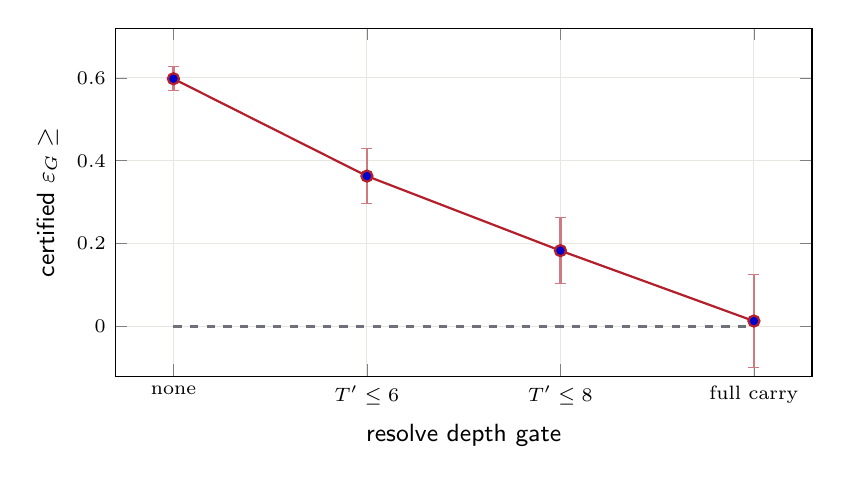
\begin{tikzpicture}
\begin{axis}[
  width=0.86\textwidth, height=60mm,
  xlabel={resolve depth gate}, ylabel={certified $\epsG\ge$},
  symbolic x coords={none, $T'\le6$, $T'\le8$, full carry},
  xtick=data, ymin=-0.12, ymax=0.72,
  grid=major, grid style={rblight},
  tick label style={font=\scriptsize},
  label style={font=\small\sffamily},
]
\addplot+[color=rbred, thick, mark=*, mark size=2pt,
  error bars/.cd, y dir=both, y explicit,
  error bar style={color=rbred!60, thick}]
  coordinates {
    (none, 0.598) +- (0.028, 0.029)
    ($T'\le6$, 0.363) +- (0.062, 0.067)
    ($T'\le8$, 0.183) +- (0.078, 0.079)
    (full carry, 0.013) +- (0.113, 0.112)
  };
\addplot[color=rbgrey, dashed, thick]
  coordinates {(none,0) (full carry,0)};
\end{axis}
\end{tikzpicture}
\caption{The dose-response of belief carrying. Each point is a
certified lower bound on $\epsG$ from the probe family (mirrored
seeds, Wilson 95\% intervals): $0.598$ with no carrying (the stored
profile, Paper~II), $0.363$ resolving only boundaries at $T'\le6$
($0.97$\,s/resolve), $0.183$ at $T'\le8$ ($3.3$\,s/resolve), and
$0.013\ [-0.10,+0.13]$ with full carrying ($\approx4.9$\,s/resolve,
$5.8$ resolves/game). As far as this instrument can see, the belief
reset was the whole of the measured exploitability.}
\label{fig:dose}
\end{figure}

\paragraph{The two findings that define the generation.} First,
belief carrying gains \emph{nothing} head-to-head: the resolver beats
the stored profile $50.3\%\ [47.2,53.4]$ --- an equilibrium of the
correctly-believed subgame does not harvest a fixed opponent; only
best response does. Second, it is a large \emph{defensive} win
(Figure~\ref{fig:dose}). Beliefs pay in defense, not offense. The
cost anti-correlates with the benefit: the deep layers where TV is
worst ($0.92$--$0.95$) are precisely the cheapest to resolve
($\le1$\,s), which is what makes full carrying practical.

\paragraph{Why none of this certifies anything.} Three obstructions,
each fatal alone:
\begin{enumerate}\itemsep2pt
\item \textbf{Unsafe re-solving has no theorem.} Each resolve derives
      $\mu_h$ assuming the agent's own past strategy; an opponent who
      knows this can deviate early to poison the assumption and cash
      in later. Known constructions in the re-solving literature make
      naive re-solving strictly \emph{more} exploitable. Our probe
      found no such attack --- which is evidence about the probe.
\item \textbf{The filter's opponent transfer is a model}
      (Section~\ref{sec:filter}); a guarantee must hold against
      opponents no filter models.
\item \textbf{The leaves are $\gp$-flavored.} Every resolve prices
      its exits with stored values computed under class priors at
      deeper boundaries; their error \emph{as $\game$-values} is the
      dominant unknown --- and Section~\ref{sec:frontier} measures it
      as substantial ($0.146$ worst-case at $T'{=}3$).
\end{enumerate}
The structural inequality
$\epsG \le \varepsilon_{\mathrm{comp}} + 2U\cdot\mathbb{E}[\mathrm{TV}]\cdot\mathrm{depth}$
is vacuous at $\mathrm{TV}=0.842$ (right side $\approx10$ against a
trivial cap of $2$) and does not touch obstruction~1 at all. So the
certificate requires a different agent --- the one the theorem of
Section~\ref{sec:theorem} is about.

\section{The safe-resolving gadget}\label{sec:gadget}

Fix the agent seat $p$ and opponent $q$. All values are seat-0 payoffs
in $[-1,1]$; $U=2$ is the payoff range. A boundary $b$ is a full
public history ending at a procurement resolution; $\kappa(b)$ its
class, $g_b$ the agent's exact own tilt there, $K_b$ the class's
deal-coupling kernel. The agent plays the stored root solve at the
game root, and at every boundary it reaches, the strategy extracted
from the gadget solve below; the \emph{leaf functional}
$\hat v_b(b',s',t')\in[-1,1]$ prices round-end leaves (currently the
stored values; Section~\ref{sec:frontier} upgrades them), and terminal
leaves are exact.

\begin{definition}[Safe-resolving gadget]\label{def:gadget}
At boundary $b$ with own range $g_b$ and any strictly positive
weighting $\nu_b$ on the opponent's types, the gadget game
$\tilde G(b)$ is: chance draws $(s,t)$ with weight
$K_b(s,t)\,g_b(s)\,\nu_b(t)$; the opponent observes $t$ and chooses
\textsc{out}, ending the game at the \emph{promise} $w_b(s,t)$, or
\textsc{in}, after which the one-round subgame of $\kappa(b)$ is
played with leaves priced by $\hat v_b$. The agent never opts out.
\end{definition}

Define the conditional promise
$\hat w_b(t) := \sum_s K_b(s,t)\,g_b(s)\,w_b(s,t) \,/\, M_b(t)$ with
$M_b(t) := \sum_s K_b(s,t)\,g_b(s)$, and for any agent round strategy
$\sigma$ and opponent behavior $\tau$ the opponent's conditional
counterfactual value $\tilde V^{\tau}_q(b,t;\sigma)$ in the gadget.
The weighting $\nu_b$ cancels from every conditional quantity; it
tunes convergence only.

\begin{lemma}[Margin identity]\label{lem:margin}
Let $\sigma_b$ be the agent's average strategy from the gadget solve
and $m_b(t) := \max_{\tau} \tilde V^{\tau}_q(b,t;\sigma_b) - \hat w_b(t)$
its measured per-type margin (one exact best-response sweep, recorded
live). Then $m_b(t)\ge0$, and every opponent behavior in the gadget
satisfies $\tilde V^{\tau}_q(b,t;\sigma_b) \le \hat w_b(t)+m_b(t)$.
\end{lemma}

\begin{proof}
The best response includes \textsc{out}, whose conditional value is
exactly $\hat w_b(t)$, so the maximum is at least $\hat w_b(t)$; the
inequality is the definition of the maximum. The sweep is exact: the
opponent's in-round information sets are (public node, private state)
pairs, swept by per-state argmax against path-summed agent reach, then
a per-type maximum over pre-stage choices including \textsc{out}.
\end{proof}

\begin{lemma}[Carry-down consistency]\label{lem:carry}
Construct promises and prices from \emph{one} functional $\hat v$: at
every resolve, $w_b := \hat v$ on the entry grid of $\kappa(b)$, and
leaves priced by $\hat v_b$. If $b'$ is a successor boundary reached
from the resolve at $b$, with $g_{b'}$ the played-strategy transfer of
$g_b$, then the conditional promise of the next resolve equals the
conditional leaf price the $b$-resolve charged:
$\hat w_{b'}(t') = \sum_{s'} K_{b'}g_{b'}\hat v_b(b',s',t')/M_{b'}(t')$.
\end{lemma}

\begin{proof}
Both sides are the same $g_{b'}$-weighted average of the same matrix:
the filter propagates its own factor under exactly the played strategy
(the byte-exact shadow gate), and the opponent factor cancels from the
conditional by Lemma~\ref{lem:cond}. Verified as a float-precision
identity on played traces.
\end{proof}

\begin{remark}[One-sidedness, and why it matters]\label{rem:oneside}
Lemma~\ref{lem:carry} is an equality for the one-functional
construction, but the telescoping argument below survives promises
\emph{at or below} the parent's leaf conditionals --- a promise may be
tightened downward without breaking soundness. This freedom is what
the ``hybrid'' promise experiments of Section~\ref{sec:ledger} price,
and its measured failure mode (tightening without enforcement is
harmful) is one of the program's sharpest lessons.
\end{remark}

Implementation status, all gates green: prior-weight gadget solve
reproduces the stored value (margins under $20\times$ solver
tolerance); the compiled kernel and the reference implementation agree
on the gadget game to $10^{-9}$ at identical iteration counts; safe
shadow replay is byte-exact ($10^{-12}$); full games run with zero
fallbacks, including forced filter-break survival; and the gadget's
conservatism costs $-1.4$ percentage points head-to-head against the
unsafe resolver (CIs overlapping) at $\varepsilon_{\max}=8.9\times10^{-4}$
per resolve.

\section{The composition theorem}\label{sec:theorem}

\begin{assumption}\label{ass:full}
Full carry: every non-terminal boundary the agent reaches is resolved.
A depth-gated agent adds, per unresolved round, an uncertified
belief-reset term; the certificate is a full-carry object.
\end{assumption}

\begin{assumption}\label{ass:break}
No unrepaired filter break --- enforced by construction in safe mode
(Section~\ref{sec:filter}); the repair preserves every conditional the
certificate consumes and cannot itself break.
\end{assumption}

For opponent type $t$ at reachable boundary $b$, let $\CBV_A(b,t)$ be
the supremum over opponent play below $b$ of the opponent's true
conditional counterfactual value in $\game$ against the agent's
continuation, with the $K_b(\cdot,t)\,g_b$ counterfactual weighting.
Reachable chains are sequences $(b_1,t_1)\to\cdots\to(b_L,t_L)$ of
successor boundaries and opponent types under the agent's public
dynamics; a game has at most $L_{\max}=8$ resolved boundaries
($T'=9,\dots,2$; re-derived by script).

\begin{theorem}[Composition, measured form]\label{thm:comp}
Under Assumptions~\ref{ass:full} and~\ref{ass:break}, for every
opponent strategy $\tau$:
\[
u_q(A,\tau) \;\le\; B^{\mathrm{root}}_q \;+\;
\pathmax{(b_1,t_1)\to\cdots\to(b_L,t_L)}\;\sum_{i=1}^{L} m_{b_i}(t_i),
\]
where $B^{\mathrm{root}}_q$ is the opponent's exact best-response value
against the stored root tables in the $\hat v$-priced root round, and
the maximum ranges over reachable chains. For the mirrored agent pair,
$\varepsilon_{\mathrm{pair}} \le
\varepsilon_{\mathrm{round}}(\mathrm{root}) +
\sum_{\mathrm{seats}}\pathmax{\mathrm{chains}}\sum_i m_{b_i}(t_i)$.
\end{theorem}

\begin{proof}
Bottom-up induction on boundaries with
$D(b,t) := m_b(t) + \max_{(b',t')\text{ reachable}} D(b',t')$ (empty
max $=0$); the claim is $\CBV_A(b,t)\le\hat w_b(t)+D(b,t)$.

\emph{Base}: a resolve whose leaves are all terminal has $\hat v$
exact, so the gadget \emph{is} the truth below $b$ restricted to
\textsc{in}, and Lemma~\ref{lem:margin} closes it.

\emph{Step}: fix $\tau$ below $b$. The true conditional value
decomposes over the round's leaf aggregates: writing $\rho_\tau$ for
opponent-and-chance reach into the aggregate landing on $(b',t')$,
\[
V^{\tau}_q(b,t) = \tilde V^{\tau}_q(b,t;\sigma_b)
+ \sum_{(b',t')} \rho_\tau\Bigl[\,V^{\tau}_q(b',t')
- \tfrac{\sum_{s'}K_{b'}g_{b'}\hat v_b(b',s',t')}{M_{b'}(t')}\Bigr],
\]
because gadget and truth differ only in leaf pricing, and the agent's
reach into each leaf under $\sigma_b$ is exactly what defines
$g_{b'}$. By Lemma~\ref{lem:carry} the subtracted term is
$\hat w_{b'}(t')$; by induction the bracket is at most $D(b',t')$;
by Lemma~\ref{lem:margin} the first term is at most
$\hat w_b(t)+m_b(t)$. Take suprema.

\emph{Root}: the same decomposition applied once to the stored root
round, prior-weighted over root types, plus the zero-sum meter
identity $B^{\mathrm{root}}_0+B^{\mathrm{root}}_1 =
\varepsilon_{\mathrm{round}}(\mathrm{root})$.
\end{proof}

\begin{remark}
The bound is opponent-model-free: the weighting $\nu_b$ and the
filtered opponent factor influence which equilibrium the resolve finds
--- hence how small the margins come out --- never the validity of the
theorem. This is exactly the property unsafe re-solving lacks.
\end{remark}

End-to-end verification: the composed two-level agent (gadget resolve
at a $T'{=}3$ boundary plus per-history gadget resolves at its
$T'{=}2$ successors) is transcribed into the flattened perfect-recall
oracle, the opponent is exact-best-responded per type, and the result
is checked against $\hat w$ plus the chain-sum of recorded margins ---
5/5 configurations pass (both seats, prior and tilted entries,
including the worst promise-dishonor class); carry-down consistency
holds to $3\times10^{-16}$.

\section{The exact frontier}\label{sec:frontier}

The theorem charges margins; margins are small only where promises are
\emph{honorable} --- backed by something true in $\game$. The stored
values are not: at $T'{=}3$, $37$ of $66$ class values sit outside
their exact-in-$\game$ brackets, worst case $0.146$ (stored $-0.657$
against exact $-0.510\ [-0.5105,-0.5100]$), reach-weighted
$1.36\times10^{-2}$ --- the within-subgame belief-reset composition
error, in agreement with the full-carry probe residual ($0.013$), a
satisfying cross-instrument consistency. So the certificate needs a
new object: exact values of class subgames \emph{as functions of entry
belief}.

\paragraph{The domain correction.} $V(\kappa,\mu)$ is not a function
on the full belief simplex and is not piecewise-linear there. By
Paper~I's factorization the reachable domain is the rank-one family,
and restricted to it $V$ is piecewise-\emph{bilinear} in the tilt pair
$(g_0,g_1)$: concave piecewise-linear in each tilt with the other
fixed. A facet census confirmed the model: across sampled seat
segments the worst midpoint-above-chord excess is negative (every
midpoint at least $1.4\times10^{-3}$ below chord plus certified
slack).

\paragraph{The facet census.} The operational complexity measure is
the size of a greedy \emph{strategy-library cover}: solved round
strategies such that exact best-response sandwiches (lower and upper
envelopes over library entries) close to $10^{-3}$ over a set of
candidate beliefs. Full population at $T'\le3$:

\begin{center}\small
\begin{tabular}{@{}lrr@{}}
\toprule
 & $T'=2$ & $T'=3$\\
\midrule
classes (canonical, pending-discard) & $18$ & $66$\\
library size min / median / max & $1$ / $29$ / $40$ & $1$ / $28.5$ / $47$\\
residual cover gap (max) & $8.1\times10^{-4}$ & $9.9\times10^{-4}$\\
holdout gap median / max & $2.3\times10^{-3}$ / $0.196$ & $4.5\times10^{-3}$ / $0.657$\\
stored value outside exact bracket & $0/18$ & $37/66$\\
stored-minus-exact delta, median / max & $1.2\times10^{-4}$ / $2.0\times10^{-4}$ & $4.3\times10^{-4}$ / $0.146$\\
\bottomrule
\end{tabular}
\end{center}

Facet counts are tens per class against a kill criterion of $10^{5}$:
the exact frontier is cheap where it was feared expensive. $T'{=}2$
stored values are exact in $\game$ ($18/18$ inside brackets) --- the
layer where $\gp=\game$, confirmed. Covers are dense where mass goes
and weak at belief-space vertices (holdout max $0.657$), which
returns with force below. At $T'{=}4$, buildability and reach
\emph{anti-correlate}: the most-visited classes exceed flat-tree build
budgets, so deep-layer certification leans on functional pricing at
$T'{=}5$ boundaries rather than exact $T'{=}4$ leaves for the heavy
classes. Frontier validation is oracle-, mirror- and
$T'{=}2$-containment-based; stored-value equality is \emph{not} a gate
above $T'{=}2$, by the measurement above.

\paragraph{What the frontier owes the certificate.} The theorem
quantifies over all opponents, including ones steering to boundaries
no probe visits, so the certificate needs an a-priori bound on
$m_b(t)$ valid at every reachable $(b,g_b)$. Per gated class $\kappa$
and every member $g$ of its factored entry family, items in force:
(1) an \emph{honorable promise vector} $w_\kappa(g,\cdot)$ --- a
certified guarantee that some playable library strategy caps the
opponent's true conditional CFV below the boundary at
$w_\kappa(g,t)+r_\kappa(g,t)$ for all $t$ simultaneously, with
certified residual $r$; (2) the \emph{functional sandwich gap}
$\Delta_\kappa(g,t)$ between the library's envelopes evaluated at the
resolve's own entry ranges (two exact-BR sweeps per entry,
$\sim$5\,ms) --- the leaf-error norm of record; (3) an \emph{off-path
enforcement rule}: the resolver compares its solve's measured margins
against the capping entry's and plays the better, converting measured
margins into the a-priori form
$m_b(t)\le\varepsilon_b+r_{\kappa(b)}(g_b,t)$.

\begin{corollary}[Certified form]\label{cor:cert}
With (1)--(3) in place,
$\varepsilon_{\mathrm{pair}} \le
\varepsilon_{\mathrm{round}}(\mathrm{root}) +
\sum_{\mathrm{seats}}\pathmax{\mathrm{chains}}
\sum_{i=1}^{L\le L_{\max}}
[\,\varepsilon_{b_i} + r_{\kappa(b_i)}(g_{b_i},t_i)\,]$,
every term computed offline or recorded live.
\end{corollary}

\section{The ledger, and the audited verdict}\label{sec:ledger}

Everything above exists in code with green gates. This section reports
what happens when it is all assembled --- kept deliberately close to
the project's internal ledger, because the assembly is where an
earlier draft of this program fooled itself, and the audit that caught
it is part of the result.

\paragraph{One functional, measured margins.} With the one-functional
carry-down (a single price surface: frontier prior-entry values where
covered, stored values elsewhere --- used as both leaf pricing and
promises), Lemma~\ref{lem:carry} holds by construction at every layer
and the meter isolates exactly one quantity: honorability of the price
surface.

\begin{table}[t]
\centering
\caption{Per-layer certificate terms under the one-functional
carry-down ($171$ resolves over $32$ full-carry games): mean-of-max
per-type margin plus mean resolve residual $\varepsilon_b$. The
mechanism proves itself at $T'{=}2$, where promises are exact in
$\game$ and the meter vanishes; the distance is the stored surface at
$T'\ge4$.}
\label{tab:layerterms}
\small
\begin{tabular}{@{}lrrl@{}}
\toprule
Layer & margin (mean-of-max / max) & $\varepsilon_b$ (mean) & price surface\\
\midrule
$T'{=}9$ & $0.134$ / $0.363$ & $9.3\times10^{-4}$ & stored\\
$T'{=}8$ & $0.133$ / $0.734$ & $9.1\times10^{-4}$ & stored\\
$T'{=}7$ & $0.111$ / $0.508$ & $8.7\times10^{-4}$ & stored\\
$T'{=}6$ & $0.106$ / $0.310$ & $2.1\times10^{-4}$ & stored\\
$T'{=}5$ & $0.148$ / $0.900$ & $2.4\times10^{-4}$ & stored\\
$T'{=}4$ & $\mathbf{0.258}$ / $0.790$ & $9.1\times10^{-5}$ & stored (libraries landing)\\
$T'{=}3$ & $0.085$ / $0.499$ & $9.6\times10^{-5}$ & frontier (prior point)\\
$T'{=}2$ & $\mathbf{0.0003}$ / $0.0006$ & $1.7\times10^{-4}$ & frontier --- \emph{honorable}\\
\bottomrule
\end{tabular}
\end{table}

Table~\ref{tab:layerterms} carries the whole story. Where the surface
is honorable ($T'{=}2$: terminal-exact frontier values) the margin
term collapses to gap scale --- the certificate mechanism works.
Where it is the stored surface ($T'\ge4$) each resolve charges
$0.11$--$0.26$, and layers $4$--$9$ carry $91\%$ of the per-seat
chain. Resolve residuals ($10^{-4}$ scale) are irrelevant everywhere:
there is nothing to buy by solving harder.

\begin{incident}{the 1.958 that was not a bound (2026-08-03)}
Summing Table~\ref{tab:layerterms}'s on-path terms over $L_{\max}=8$
and both seats gives $1.958$ --- and an earlier draft of this ledger
reported it as the certificate. An independent adversarial audit
rejected it: the theorem's chain maximum ranges over
\emph{opponent-steerable} chains, and an on-path mean substitutes a
self-play average for a supremum the opponent controls. The licensed
assembly from the same data --- worst observed chain over visited
boundaries only --- is $8.22$: vacuous. Reach-weighting is not a sound
repair (the opponent steers the carried beliefs; self-play samples a
measure-zero slice of the chain space). The audit's verdict, adopted
in full: \textbf{certified $\epsG$ today is the trivial cap}. The
sound averaging opportunities that survive --- root-prior weighting
over the opponent's root type, and a chance-expectation reproof of the
successor step (the verification's $0.4$--$2.0$ slack locates the
loose inequality) --- are theorem work, listed in the program. Lesson:
in certification, the assembly is as much a proof obligation as the
per-piece inequalities, and an average is never a supremum.
\end{incident}

\paragraph{Fixed promise surfaces are certifiably dead.} The audit
also produced the program's most decisive positive tool. Per-type
dishonor of a \emph{fixed} promise surface is linear-fractional in the
own tilt, so its supremum over the rank-one family is attained at
own-type vertices and can be certified exactly (a clairvoyant best
response per vertex). Result: the func surface's certified sup
dishonor is median $\approx1.0$, max $2.0$, at \emph{both} $T'{=}2$
and $T'{=}3$ --- even where on-path margins measure $3\times10^{-4}$.
An earlier holdout measurement suggesting fixed refined surfaces might
suffice (max $0.063$) was a sampling artifact of insufficiently
extreme tilts. Any certificate path through a fixed promise matrix is
closed, permanently, at every layer; what remains open is
\emph{range-dependent} promises (library caps evaluated at the
realized entry range) with per-type enforcement, whose residual is the
library sandwich-gap supremum --- itself lower-bounded by vertex
probes at $0.14$--$0.43$ median today, hence the vertex-completion
item in the program.

\paragraph{Enforcement is mandatory, not optional.} Honorable
(tighter) promises push opponent opt-out mass up, and CFR's weighted
objective then simply ignores opted-out types --- their margins are
only weakly controlled by the solve. Measured: hybrid promises
(tightened by Remark~\ref{rem:oneside}) \emph{worsen} the $T'{=}3$
margin term from $0.085$ to $0.634$ as built, because the meter
measures against the tighter bar while the solve stops defending it.
The audit's a-priori judgment (``sound but worthless without
enforcement'') was generous; the measurement says actively harmful.
Post-solve per-type minimization with the capping entry --- item (3)
above --- is load-bearing machinery.

\paragraph{The sandwich at window close.}

\begin{table}[h]
\centering
\caption{The certificate scoreboard. Lower bounds are probe results
(mirrored seeds, $n=300$ games, Wilson 95\%); the upper bound is the
audited assembly status. The ship gate is $0.10$.}
\label{tab:sandwich}
\small
\begin{tabular}{@{}lr@{}}
\toprule
Instrument & value\\
\midrule
probe LB, unsafe full carry & $\epsG \ge 0.013\ [-0.10,\,+0.13]$\\
probe LB, safe + stored promises & $\epsG \ge 0.160\ [0.047,\,0.269]$\\
probe LB, safe + certified $T'\le3$ promises & $\epsG \ge 0.113\ [0.000,\,0.224]$\\
certificate UB (audited) & \textbf{trivial ($2.0$)}\\
\bottomrule
\end{tabular}
\end{table}

Two readings of Table~\ref{tab:sandwich} matter. The safe agent with
dishonorable stored promises is \emph{measurably more exploitable}
($0.160$) than the unsafe agent ($0.013$): safety machinery with bad
promises is worse than no machinery, because the opponent can farm the
dishonor --- the probe converts exactly the margins of
Table~\ref{tab:layerterms} into realized wins, which confirms the
dishonor is substance, not accounting. And certified promises at
$T'\le3$ move the point estimate in the right direction ($0.160\to
0.113$) but $n=300$ cannot separate them; the certificate's upper
bound, not more probe games, is the instrument of record --- a
deliberate allocation choice, since separating the variants at $95\%$
costs $10$--$20$k games of compute that certifies nothing.

\section{The program}\label{sec:program}

Four items, each with the measurement that motivates it, in
dependency order. The generation's risk is concentrated in item~2.

\begin{enumerate}\itemsep3pt
\item \textbf{Vertex-complete frontier libraries at $T'\le4$.} One
      exact solve per feasible own-type vertex ($10$--$144$ per class,
      sub-second each) collapses the library gap at vertices to solve
      tolerance; the interior sup then follows from the
      piecewise-bilinear structure by small bilinear programs.
      Target: certified per-class residual $r_\kappa$ at $T'\le4$ of
      order $5\times10^{-3}$. Engineering plus modest theory; the
      vertex probes above say the gap is real and say exactly where.
\item \textbf{Certified cap propagation upward.} A $T'{\ge}5$ cap
      against a strategy is one kernel exact-BR round sweep with
      capped leaves --- sound by Theorem~\ref{thm:comp}'s machinery.
      The open question is whether six layers of propagation stay
      tight; the measured evidence for hope is that interval
      propagation \emph{contracts} per layer ($0.66$--$1.03\times$,
      round mixing diluting leaf error) rather than fattening. This is
      the research risk of the generation, and it is
      measurement-first testable in days.
\item \textbf{Enforcement transcription.} Library entries transcribed
      to playable round strategies; per-type minimization at resolve
      time. Converts measured margins into a-priori bounds and flips
      the hybrid experiment from harmful to a strict win.
\item \textbf{Sound accounting.} The audit's surviving averaging
      opportunities: margin de-duplication (measured $-0.007$),
      $a$-invariant chain assembly (per-type margin vectors are
      persisted for exactly this), root-prior weighting, and the
      chance-expectation reproof of the successor step.
\end{enumerate}

Probe power is a compute line item only after items 1--3 move the
certificate; the sandwich's upper jaw is where the next result lives.

\paragraph{Out of scope.} Serving latency (the resolve-service versus
belief-bucket question), multiplayer, public-statistic enrichment
(dead by Paper~II's refinement ladder), further equilibrium-set
selection (real-game noise by Paper~II's measurements).

\section{Verification}\label{sec:verification}

House rule, unchanged from Papers~I--II: no number enters this paper
without a script that regenerates it. \code{v6\_verify\_composition.py}
re-derives $L_{\max}$, checks Lemma~\ref{lem:carry} as a
float-precision identity on played traces, and verifies
Theorem~\ref{thm:comp} end-to-end against the perfect-recall oracle on
composed two-level agents (5/5 configurations). The filter, gadget,
shadow-replay, filter-break and kernel-parity gates run in the
simulator's test suite; the facet census, fattening, margin-by-layer,
vertex-sup and probe measurements each write a JSON artifact whose
values appear here verbatim. The perfect-recall oracle merges
procurement flip interleavings (order irrelevance, Paper~I), so the
verified agent variant feeds its filter order-canonicalized records;
this changes nothing in the theorem, which never references flip
order.

\bigskip
\noindent\emph{Status line, for the reader who skipped to the end:
the theorem is proved, the machinery is built and gated, the lower
jaw is at $0.013$, the upper jaw is trivial, and the entire distance
is one named quantity --- honorability of the price surface at
$T'\ge4$ --- with a four-item program aimed at it.}

\end{document}
